\chapter{Исследовательская часть}

В данном разделе будут приведены примеры работы программ, постановка эксперимента и сравнительный анализ алгоритмов на основе полученных данных.

\section{Технические характеристики}

Технические характеристики устройства, на котором выполнялось исследование.

\begin{enumerate}
	\item Операционная система: Windows 10 Корпоративная, Версия	21H1, Сборка ОС 19043.2006.
	\item Оперативная память: 8 ГБ.
	\item Процессор: AMD Ryzen 5 4600H с видеокартой Radeon Graphics \\3.00 ГГц \cite{processor}.
\end{enumerate}

Исследование проводилось на ноутбуке, включенном в сеть электропитания. 
Во время исследования ноутбук был нагружен только встроенными приложениями окружения, а также непосредственно системой.

\section{Демонстрация работы программы}

На рисунке \ref{fig:democonsole} представлены результаты работы реализаций алгоритма полного перебора и муравьиного алгоритма.
\captionsetup{justification=centering, singlelinecheck=false}
\begin{figure}[H]
	\centering
	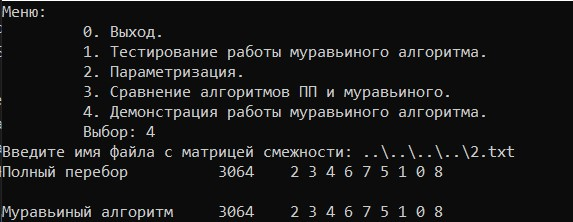
\includegraphics[width=1\linewidth]{inc/img/democonsole}
	\caption{Демонстрация работы программы в консоли}
	\label{fig:democonsole}
\end{figure}

\section{Параметризация метода}

Для проведения параметризации были использованы матрицы смежности \eqref{matrix1}, \eqref{matrix2}, \eqref{matrix3}. 
В качестве класса данных была выбрана карта перемещения по портам через океаны.
Матрицы смежности для выбранного класса данных:

\begin{equation}
	\hspace*{-0.5mm}\label{matrix1}
	M_1 = \begin{pmatrix}
		0	&681	&335	&725	&1215	&657	&210	&1325	&372	&227\\
		681	&0	&675	&152	&1537	&1080	&886	&1494	&694	&454\\
		335	&675	&0	&827	&1547	&405	&364	&1660	&704	&518\\
		725	&152	&827	&0	&1470	&1232	&930	&1373	&657	&498\\
		1215	&1537	&1547	&1470	&0	&1825	&1378	&580	&843	&1136\\
		657	&1080	&405	&1232	&1825	&0	&447	&1949	&982	&879\\
		210	&886	&364	&930	&1378	&447	&0	&1502	&535	&432\\
		1325	&1494	&1660	&1373	&580	&1949	&1502	&0	&967	&1204\\
		372	&694	&704	&657	&843	&982	&535	&967	&0	&293\\
		227	&454	&518	&498	&1136	&879	&432	&1204	&293	&0\\
	\end{pmatrix}
\end{equation}

\begin{equation}
	\label{matrix2}
	M_2 = \begin{pmatrix}
0	&140	&1194	&1362	&688	&167	&481	&220	&325\\
140	&0	&1054	&1277	&640	&185	&341	&154	&382\\
1194	&1054	&0	&784	&731	&1164	&749	&997	&1436\\
1362	&1277	&784	&0	&674	&1306	&1048	&1169	&1659\\
688	&640	&731	&674	&0	&632	&505	&495	&1002\\
167	&185	&1164	&1306	&632	&0	&451	&167	&492\\
481	&341	&749	&1048	&505	&451	&0	&284	&723\\
220	&154	&997	&1169	&495	&167	&284	&0	&507\\
325	&382	&1436	&1659	&1002	&492	&723	&507	&0\\
	\end{pmatrix}
\end{equation}


\begin{equation}
	\label{matrix3}
	M_3 = \begin{pmatrix}
	0	&1726	&541	&139	&744	&829	&361	&447	&1278\\
	1726	&0	&2149	&1865	&2173	&1969	&2087	&1904	&2864\\
	541	&2149	&0	&402	&389	&710	&182	&741	&785\\
	139	&1865	&402	&0	&629	&838	&222	&400	&1139\\
	744	&2173	&389	&629	&0	&330	&543	&1029	&951\\
	829	&1969	&710	&838	&330	&0	&849	&1238	&1272\\
	361	&2087	&182	&222	&543	&849	&0	&559	&917\\
	447	&1904	&741	&400	&1029	&1238	&559	&0	&1370\\
	1278	&2864	&785	&1139	&951	&1272	&917	&1370	&0\\
	\end{pmatrix}
\end{equation}

Первый столбец представляет собой значения параметра $t_{max}$, второй --- $\alpha$, третий --- $\rho$, в четвертом столбце представлено максимальное отклонение длины маршрута, полученного методом на основе муравьиного алгоритма, от оптимальной длины маршрута, вычисленной методом полного перебора, в пятом --- отклонение медианы.

Для каждой комбинации параметров, муравьиный алгоритм запускался по 30 раз (для каждой матрицы 10 раз). 
Для каждого из 30 полученных значений вычислялось отклонение от наилучшего маршрута. Для таблицы выбирались максимальное значение отклонения и медианное.

Как видно из таблицы \ref{tbl:param}, наилучшим значением настроечного параметра $\alpha$ является значение, равное 0.5, а коэффициента испарения $\rho$ ---  0.1. Уже при $t_{max} = 500$ все медианные отклонения равны нулю.

\section{Время выполнения реализаций алгоритмов}

Замеры времени для каждого количества количества вершин в графе проводились 20 раз. 
В качестве результата взято среднее время работы алгоритма на данном количества вершин при следующих параметрах: $\alpha = 0.5$, $\rho = 0.5$, $ t_{max} = 500$.

Результаты замеров времени приведены в таблице \ref{tab:time}.
На рисунке \ref{fig:time}, приведена зависимость времени работы реализаций алгоритмов. 
\captionsetup{justification=raggedright,singlelinecheck=false}
\begin{table}[H]
	\begin{center}
		\caption{\label{tab:time}Время выполнения реализаций алгоритма полного перебора и муравьиного алгоритма}
		\begin{tabular}{|c|d|d|}
			\hline
			Количество вершин & \multicolumn{1}{c|}{Муравьиный алгоритм, мс} & \multicolumn{1}{c|}{Полный перебор, мс} \\\hline
			5	&	12.500	&	0.000	\\\hline
			6	&	20.313	&	1.563	\\\hline
			7	&	33.594	&	9.375	\\\hline
			8	&	50.781	&	90.625	\\\hline
			9	&	73.438	&	1007.813	\\\hline
			10	&	96.094	&	10689.063	\\\hline
		\end{tabular}
	\end{center}
\end{table}
\captionsetup{justification=centering,singlelinecheck=false}
\begin{figure}[H]
	\centering
	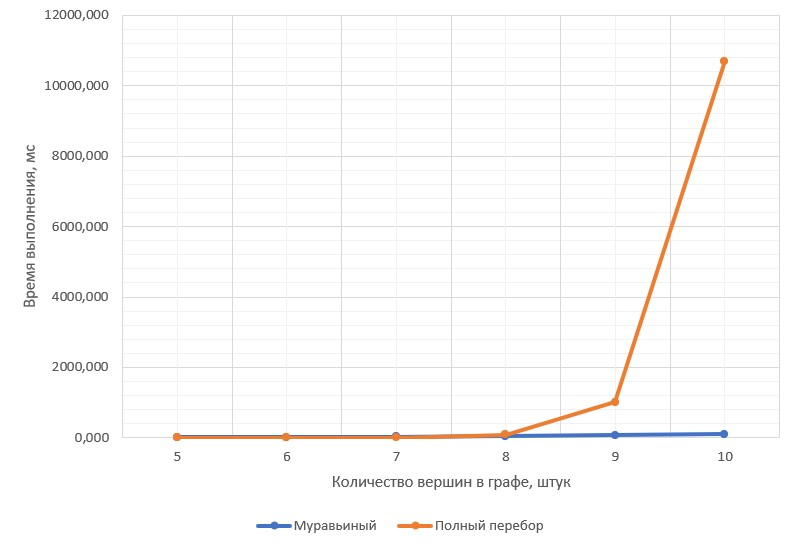
\includegraphics{inc/img/time}
	\caption{Зависимость времени работы реализаций алгоритма полного перебора и муравьиного алгоритма}
	\label{fig:time}
\end{figure}

Как можно наблюдать на графике, время работы алгоритма полного перебора растет экспоненциально в зависимости от размера матрицы смежности, в отличие от муравьиного алгоритма, время которого изменяется практически линейно.

\section{Оценка трудоёмкости}



Алгоритм полного перебора имеет факториальную сложность, т.к. количество всех маршрутов равно числу размещений из $n$ городов.
\begin{equation}
	A_n = n!
\end{equation}

Следовательно сложность метода полного перебора $O(n!)$

Сложность муравьиного алгоритма равна $O(t_{max}\cdot n^2 \cdot m)$, где $t_{max}$ --- время жизни колонии, $m$ --- количество муравьев в колонии, $n$ --- количество точек в графе.

\begin{itemize}[label=---]
	\item $f_{\text{утро}} =  6 +  9n       + 5n^2$
	\item $f_{\text{день}} =	    n - 39m          + 24mn + 15mn^2 $
	\item $f_{\text{закат}} = 5 + 19n + 7m           + 4mn$
	\item $f_{\text{ночь}} =  1 +  3n       + 20n^2$
\end{itemize}

Итоговая трудоемкость метода на основе муравьиного алгоритма рассчитывается по формуле \eqref{eq:trud}
\begin{equation}
	\label{eq:trud}
\begin{array}{cc}
	&f_{\text{муравьиного алгоритма}} =  t_{max} \cdot (f_{\text{утро}} + f_{\text{день}} + f_{\text{закат}} + f_{\text{ночь}}) = \\ 
	&t_{max} \cdot (12 + 32n - 32m + 25n^2 + 29mn + 15mn^2)
\end{array}
\end{equation}
\section{Вывод}

В результате проведенных экспериментов были выявлены оптимальные параметры для метода на основе муравьиного алгоритма при выбранном классе эквивалентности: $\alpha = 0.5$, $\rho = 0.1$, $ t_{max} = 500$. 
Однако стоит учитывать, что чем больше значение $t_{max}$, тем больше вероятность того, что будет найден оптимальный маршрут, но при этом будет возрастать время выполнения программы. 

Также был проведен сравнительный анализ муравьиного алгоритма и алгоритма полного перебора. 
Метод полного перебора следует использовать для матриц небольшого размера (до 8) и в случае, если необходимо получить точное решение. 
В остальных случаях муравьиный алгоритм является более эффективным по времени, если достаточно получить хорошее решение по выбранной метрике (например, отклонение длины маршрута, полученного методом на основе муравьиного алгоритма, от оптимальной длины маршрута).

